\documentclass[a4paper,12pt,oneside]{book} % nie: report!


% pakiety
\usepackage{polski} % lepiej to zamiast babel!
\usepackage[utf8]{inputenc} % w razie kłopotów spróbować: \usepackage[utf8x]{inputenc}
\usepackage{fancyhdr} % nagłówki i stopki
\usepackage{indentfirst} % WAŻNE, MA BYĆ!
\usepackage[pdftex]{graphicx} % to do wstawiania rysunków
\usepackage{amsmath} % to do dodatkowych symboli, przydatne
\usepackage[pdftex,
            left=1in,right=1in,
            top=1in,bottom=1in]{geometry} % marginsy
\usepackage{amssymb} % to też do dodatkowych symboli, też przydatne
\usepackage{pdfpages}
\usepackage{lipsum}
\usepackage{multirow}
\usepackage{listings}
\usepackage{caption}
\usepackage{booktabs}
\usepackage{subcaption}
\usepackage{xcolor}
\graphicspath{ {./img/} }
\DeclareCaptionType{code}[Listing][Spis listingów] 

\definecolor{codegreen}{rgb}{0,0.6,0}
\definecolor{codegray}{rgb}{0.5,0.5,0.5}
\definecolor{codepurple}{rgb}{0.58,0,0.82}
\definecolor{backcolour}{rgb}{0.95,0.95,0.92}

\lstset{
	backgroundcolor=\color{backcolour},   
	commentstyle=\color{codegreen},
	keywordstyle=\color{magenta},
	numberstyle=\tiny\color{codegray},
	stringstyle=\color{codepurple},
	basicstyle=\ttfamily\footnotesize,
	breakatwhitespace=false,         
	breaklines=true,                 
	captionpos=b,                    
	keepspaces=true,                 
	numbers=left,                    
	numbersep=5pt,                  
	showspaces=false,                
	showstringspaces=false,
	showtabs=false,                  
	tabsize=2,
	float=h
}

% definicje nagłówków i stopek
\pagestyle{fancy}
\renewcommand{\chaptermark}[1]{\markboth{#1}{}}
\renewcommand{\sectionmark}[1]{\markright{\thesection\ #1}}
\fancyhf{}
\fancyhead[LE,RO]{\footnotesize\bfseries\thepage}
\fancyhead[LO]{\footnotesize\rightmark}
\fancyhead[RE]{\footnotesize\leftmark}
\renewcommand{\headrulewidth}{0.5pt}
\renewcommand{\footrulewidth}{0pt}
\addtolength{\headheight}{1.5pt}
\fancypagestyle{plain}{\fancyhead{}\cfoot{\footnotesize\bfseries\thepage}\renewcommand{\headrulewidth}{0pt}}


% interlinia
\linespread{1.25}


% treść
\begin{document}
\sloppy
\thispagestyle{empty}
\begin{titlepage}
	\begin{center}
		\vspace*{1cm}
		
		\Huge
		\textbf{Kompilacja Kernela Linux}
		
		\vspace{0.5cm}
		\LARGE
		Metoda stara i nowa
		
		\vspace{1.5cm}
		
		\textbf{Rafał Hrabia}\\
		\small nr indeksu 296583
		
		\vfill
		
		\vspace{0.8cm}
		
		\Large
		Informatyka I st.\\
		Uniwersytet Marii Curie-Skłodowskiej\\
		\today
		
	\end{center}
\end{titlepage}
\newpage{}

\thispagestyle{empty}
\newpage{}

\tableofcontents{}

\chapter{Przygotowanie}
\label{Przygotowanie}

W pierwszej kolejności po zalogowaniu się i przejściu do katalogu \emph{/usr/src} musimy zdobyć link do paczki z plikami źródłowymi kernela. Z racji tego, że
korzystam z wirtualnej maszyny bez interfejsu graficznego posłużę się komputerem, który hostuje maszynę wirtualną. Wchodzimy na stronę i przy użyciu menu
kontekstowego kopiujemy do schowka bezpośredni link to pliku(rys. \ref{link-copy}).

\begin{figure}[h]
	\centering
	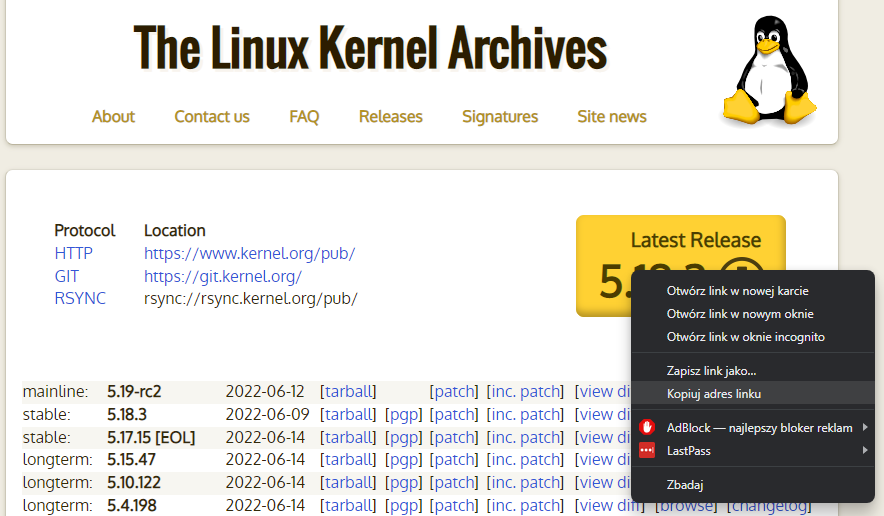
\includegraphics[scale=0.5]{01-link-copy.png}
	\caption{Kopiowanie linku}
	\label{link-copy}
\end{figure}

Do pobrania pliku jedynym słusznym wyborem będzie komenda \emph{wget}(rys. \ref{wget}).

\begin{figure}[h]
	\centering
	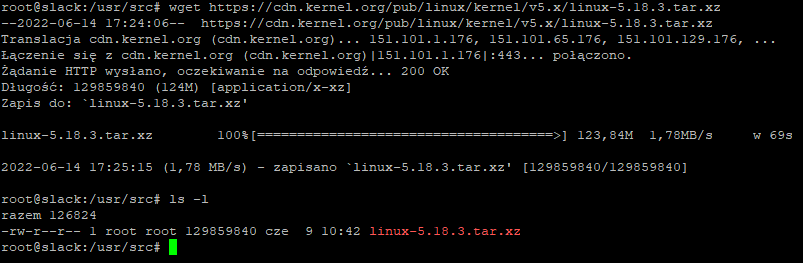
\includegraphics[scale=0.5]{02-wget}
	\caption{Pobieranie kernela}
	\label{wget}
\end{figure}

Jako, że pobrany plik jest to plik archiwum używamy na nim komendy \emph{tar -xvpf}(rys \ref{tar}).

Dla przypomnienia (flagi polecenia \emph{tar}):
\begin{itemize}
	\item x – wyodrębnia wymienione pliki
	\item v – wypisuje nazwy wszystkich plików
	\item f – określa nazwę pliku archiwum tar
	\item p - zachowuje ustawienia dostępu do plików
\end{itemize}

\begin{figure}[h]
	\centering
	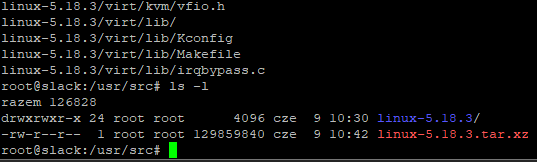
\includegraphics[scale=0.5]{03-tar}
	\caption{Rozpakowywanie archiwum}
	\label{tar}
\end{figure}

Jak można zauważyć został stworzony nowy folder zawierający pliki z archiwum.

Teraz musimy przekopiować \emph{config} znajdujący się w katalogu \emph{/proc} (rys \ref{config}). Ponieważ plik konfiguracji ma rozszerzenie wskazujące na to, że to archiwum gzip używamy polecenia \emph{zcat}.

\begin{figure}[h]
	\centering
	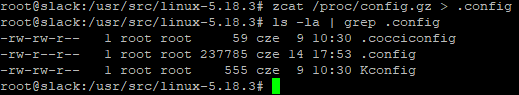
\includegraphics[scale=0.6]{04-config}
	\caption{Kopiowanie konfiguracji}
	\label{config}
\end{figure}

Przyda się zrobić kopię zapasową oryginalnego configu. W tym celu kopiujemy plik \emph{.config} do przykładowo pliku \emph{.config.bak} (rys. \ref{config-bak}).
\begin{figure}[h]
	\centering
	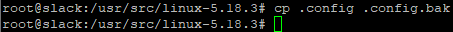
\includegraphics[scale=0.6]{05-config-bak}
	\caption{Kopia zapasowa}
	\label{config-bak}
\end{figure}

\chapter{Metoda stara}
\label{Metoda stara}

Przyszła pora na wywołanie polecenia \emph{make localmodconfig}. Po pomyślnym wykonaniu jesteśmy informowani o nadpisaniu konfiguracji do pliku \emph{.config} (rys. \ref{old-config}).

\begin{figure}[h]
	\centering
	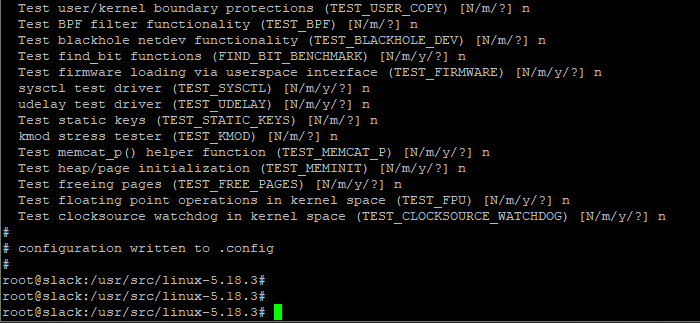
\includegraphics[scale=0.6]{06-old-config}
	\caption{Wynik polecenia \emph{make localmodconfig}}
	\label{old-config}
\end{figure}

Nastała wielka chwila - kompilacja jądra. W tym celu trzeba znowu użyć polecenia \emph{make}. Tym razem użyjemy parametru \emph{-j<liczba>} co pozwoli nam uruchomić kompilację kernela na wielu rdzeniach(lub wątkach?). W moim przypadku użyję liczby 8. 

\begin{figure}[h]
	\centering
	\includegraphics[scale=0.6]{08-bzimage}
	\caption{Kompilowanie kernela}
	\label{bzimage}
\end{figure}

\chapter{Metoda nowa}
\label{Metoda nowa}

\chapter{Wnioski}
\label{Wnioski}

%\begin{figure}[h]
%	\centering
%	\includegraphics[scale=0.4]{conv.png}
%	\caption{Warstwa konwolucyjna - zasada działania\cite{developpapercom_2021}}
%	\label{conv_img}
%\end{figure}

%\begin{lstlisting}[language=Bash, caption={}, label={}]

%\end{lstlisting}

\end{document}
